\documentclass[12pt. a4paper]{report}
\setcounter{secnumdepth}{0} % Turn off section numeration

\usepackage[utf8]{inputenc}
\usepackage[cache=false]{minted}
\usepackage{hyperref}
\usepackage{titlesec}
\usepackage{graphicx}
\graphicspath{ {./images/} }
\usepackage[section]{placeins}

\titleformat{\chapter}[display]
  {\normalfont\bfseries}{}{0pt}{\Huge}
  

\title{%
	Laboratorul numarul 1 \\
	\large Baze de date}
\author{%
	Dragomir Țurcanu \\
	\large MI-191}
\date{Decembrie 25, 2020}

\begin{document}

\definecolor{bg}{rgb}{0.95,0.95,0.95}
\setminted{
	breaklines=true,
	breakanywhere=true,
	bgcolor=bg,
	breaksymbolleft=,
	breakanywheresymbolpre=
}

\maketitle
\tableofcontents

\chapter{Sarcina}


Deoarece sarcina per-se nu a fost menționată în cadrul aplicației else, o menționez la fel cum este indicată pe website. Deci urmează de realizat însărcinarea în următorul mod.

\begin{quote}
PREZENTAREA VARIANTEI FINALE A APLICAȚIEI WEB, COMPONENTA FRONT-END SI BACK-END, PASII 1-7 CE URMA SA FIE PREZENTAT LA LABORATORUL PRECEDENT
\end{quote}

\section{Obiecivele}

\begin{itemize}
	\item Raportul PDF
	\item Prezentarea PPTX
	\item Prezentarea și zip-ul bazei de date
\end{itemize}

\section{Abordarea Proprie}
Pentru a \emph{simplifica} și în același moment de a \emph{dezvolta} ideea sarcinii, am decis să i-au ca bază laboratorul nr 6 la obiectul "Tehnologii Web", deoarece toate conceptele necesare, ba chiar mai multe sunt folosite și explicate.

Deci am mfoodificat un pic sarcina, pentru a satisface condiția. Varianta lucrării la TW, presupunea crearea unei aplicații de monitorizare și selectare a datelor referitoare la cursul valutar. Și sună în următorul mod.

\begin{quote}
De creat baza de date cu datele despre cursurile valutelor pe fiecare zi. De realizat interfaţa on-line la baza
de date cu următoarele funcţii: selectarea şi vizualizarea datelor în baza cîmpurilor diferite (denumire, data,
perioada de timp), indicarea creşterii sau scăderii cursului în perioada perioadă indicată de utilizator.
\end{quote}

\chapter{Rezolvarea}
Pentru a realiza sarcina, am decis să folosesc un set de tehnologii ce mi-ar fi interesante în lucru, și benefice pentru dezvoltarea skill-setului. De asemenea acestea au contribuit imens le menținerea interesului în dezvoltare :).

\section{Stack-ul Tehnic}
\begin{itemize}
	\item PHP 7.4
	\item MySQL 5.6
	\item Slim Framework \footnote{\url{https://www.slimframework.com/}}
	\item Doctrine ORM \footnote{\url{https://www.doctrine-project.org/projects/orm.html}}
	\item Git \footnote{\url{https://git-scm.com/}}
\end{itemize}

Apropos de Git, proiectul este disponibil deschis pe pagina mea proprie GitHub, pentru citire integrală și instrucțiuni de instalare. Accesați \href{https://github.com/dragomirt/lab6tw}{aici}, sau pe url-ul \url{https://github.com/dragomirt/lab6tw}.

\section{Concepția}
Ideea aplicației este crearea unei interfețe interactive pentru vizualizarea informației. Deoarece caracterul acestei informații este 
\emph{dinamic}, este logică folosirea tehnologiei \textbf{AJAX} \footnote{Asynchronous Javascript and XML}. 

Ținând acest fapt în considerare, am creat o singur loc de intrare, fișierul \textbf{index.html}, ce și conține toată partea vizuală, informația fiind încărcată prin requesturile \textbf{fetch} realizate de către client, pentru a trage informația din \textbf{endpointur-ile} ale \textbf{API-ului} \footnote{Application Programming Interface} intern.

Supranumitul API conține adrese pentru inserarea, modificarea, selectarea și ștergerea informației.

\section{Explicații Tehnice}

\subsection{Front End}
Așa deci, odată ce am discutat teoria, este timpul de a demonstra un pic de practică \emph{as well}. Mai jos este demonstrată aplicația în starea sa normală, pe unica pagină grafică a websiteului :D

\begin{figure}[H]
\centering
	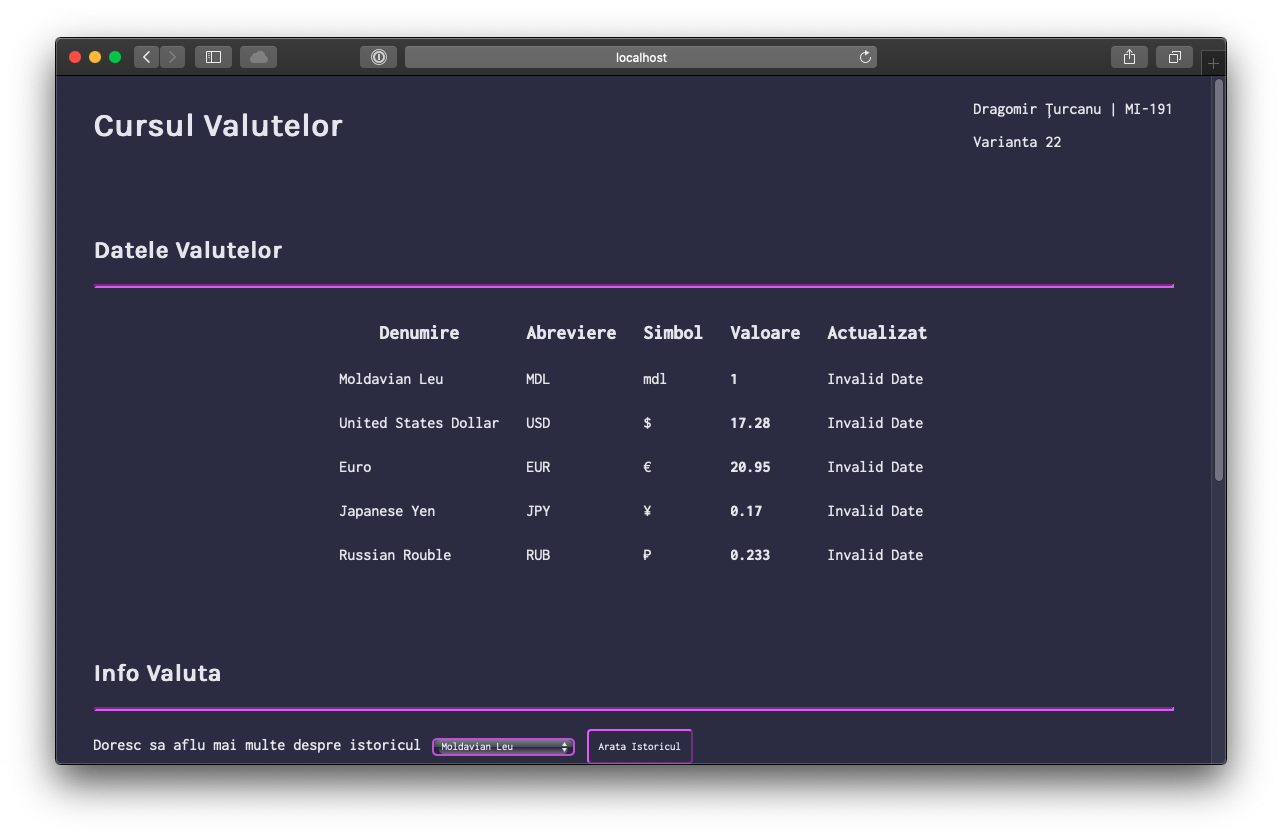
\includegraphics[width=1.0\textwidth]{homepage}
\end{figure}

Pe această pagină putem admira locul primar de interacțiune a unui utilizator de rând cu aplicația în cauză. Aici este posibilă monitorizarea și selectarea valorilor pentru citire.

Majoritatea requesturilor sunt transmise de către Javascriptul din browser în formatul următor.


\begin{minted}{javascript}
    async function getCurrencyData() {
        let response = await fetch("/api/currency");
        return await response.json();
    }
\end{minted}

Fiecare request fiind modificat pentru endpoint-ul dorit. Deci requestul de sus întoarce informații generale despre toate valutele.

Funcția întreagă ce conține requestul arată în modul următor.
\begin{minted}{javascript}
    function getAvailableCurrencies() {
        let currencySelect = document.querySelector('select#currencySelect');
        let currencySelectGraph = document.querySelector('select#currencySelectGraph');

        if (!currencySelect || !currencySelectGraph) {
            return;
        }

        currencySelect.innerHTML = "";
        currencySelectGraph.innerHTML = "";

        getCurrencyData().then(data => {
            for (const row of data) {
                availableCurrencies[row.id] = {full_name: row.full_name, symbol: row.symbol};
                currencySelect.innerHTML += `<option value="${row.id}">${row.full_name}</option>`;
                currencySelectGraph.innerHTML += `<option value="${row.id}">${row.full_name}</option>`;
            }
        });
    }
\end{minted}

Aceasta ia răspunsul requestului în format \textbf{JSON} și înscrie în pagină. La fel sunt realizate celelalte blocuri din pagină.

\subsection{Baza de date}

Baza de date în acest exemplu a fost realizată într-un mod maximal simplistic. Există 2 tabele \emph{currency} și \emph{currency\_value}.

\textbf{"currency"} presupune un tabel ce conține informație generală despre fiecare valută. Denumirea, simbolul, abrevierea și de genul. 

\textbf{"currency\_value"} la rândul său conține informație ce ține de valoarea valutei la o dată anumită. Sunt folosite chei străine secundare pentru a indica corelația între aceste 2 tabele.

Există relația One\-To\-Many la \emph{currency.id} spre\emph{\texttt{currency\_value}} și invers, Many\-To\-One pe aceleași fielduri, pentru a extrage cu ușurință informația în ambele părți.

Tot arată în modul următor.

\begin{figure}[H]
\centering
	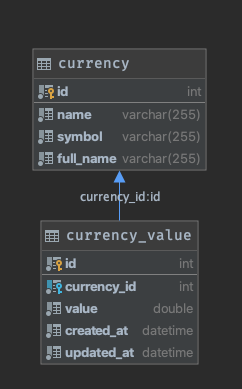
\includegraphics{database_schema}
\end{figure}
\FloatBarrier

\subsection{Back End}
Cum deja am menționat, alegerea a căzut pe \textbf{Slim Framework}. Aceasta a permis crearea rapidă a rutelor pentru API și descrierea simplă a logicii aplicației.

Spre exemplu, ruta ce întoarce datele despre valori, arată în modul următor.

\begin{minted}{php}
<?php
// Get all values
    $group->get('/currency/value', function(Request $request, Response $response) use (&$entityManager) { // Este funcția părinte ce encapsulează o funcție anonimă ce preia entityManager pentru a modifica datele cu ajutorul ORM
   
        $values = $entityManager->getRepository(CurrencyValue::class)->findBy([], ['created_at' => 'DESC']); // Sunt datele provenite din DB
        if ($values === null) { // Dacă valorile sunt nule, sfarsește funcția și întoarce un array gol ca http răspuns
            $response->getBody()->write(json_encode([]));
            return $response;
        }

        $responseFormatted = array();
        foreach ($values as $value) { // Pentru fiecare înscriere în DB, scrie datele în array-ul decodat pentru răspuns
            $responseFormatted[$value->getCurrency()->getId()][] = array(
                'value' => $value->getValue(),
                'date' => $value->getCreatedAt()
            );
        }

// Codifică răspunsul în format JSON și întoarce clientului
        $response->getBody()->write(json_encode($responseFormatted));
        return $response;
    });
?>
\end{minted}

Mai multe detalii sunt disponibile pe pagina GitHub a proiectului disponibilă mai sus.

\chapter{Concluzie}
Dezvoltarea acestui laborator a contribuit la îmbunătățirea abilităților de creare a aplicațiilor de tip API + AJAX, și a fost un proces total interesant, ce presupun că este reflectat în entuziasmul cu care prezint lucrarea. \emph{Apreciez feedbackul!}

\end{document}